\subsection{}
The provided equations for load transfer are applied on each wheel, with the respective sign convention. The roll stiffness and roll damping distributions are calculated respectively as follows:
\begin{align*}
    c_{\phi,1} &= c_{\phi} \cdot c_{\lambda}\\
    k_{\phi,1} &= k_{\phi} \cdot k_{\lambda}\\
\end{align*}

\subsection{Add roll dynamics}
The simulation is done in Simulink, and the results are in the next questions.

\subsection{Plot frequency response and coherence}
The following figures were obtained for the frequency sweep response with load transfer:

\begin{figure}[H]
    \centering
    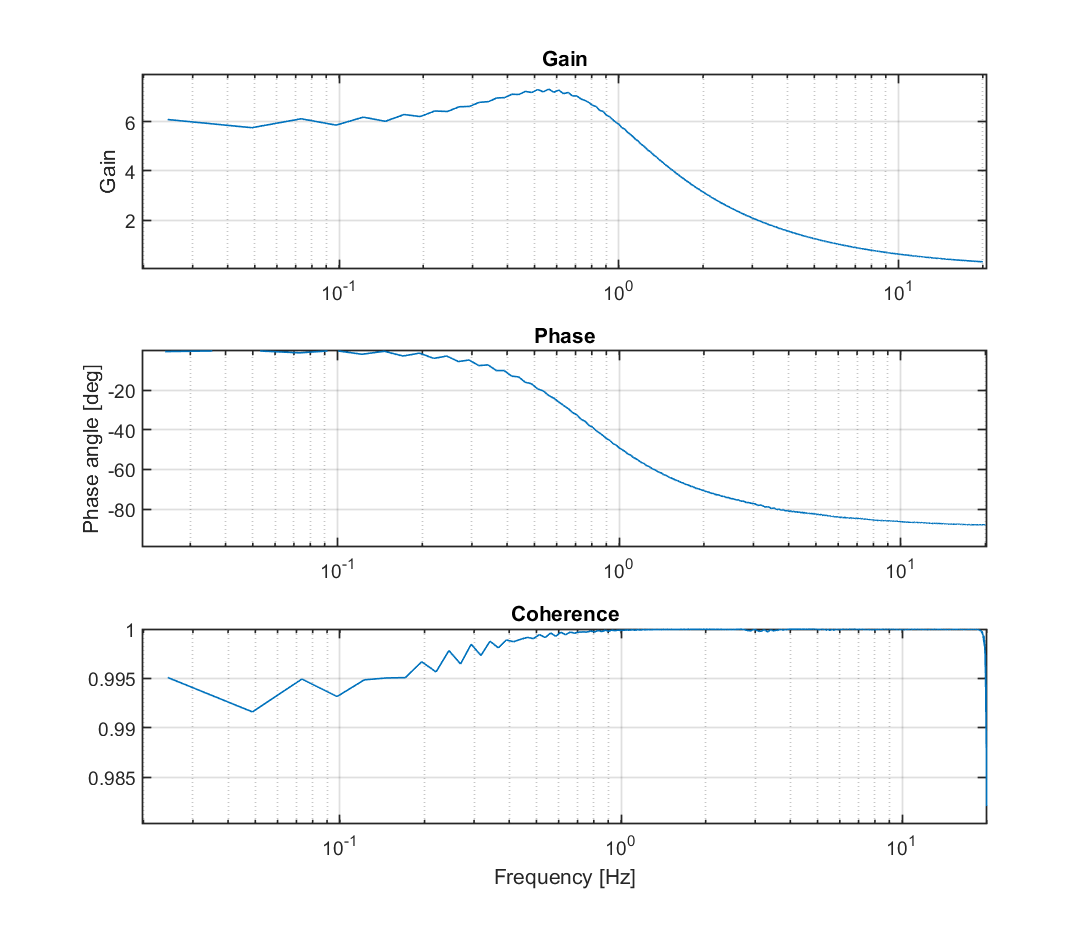
\includegraphics[width=0.8\textwidth]{Figures/2_3.png}
    \caption{Frequency Response of Vehicle with Load Transfer}
    % \label{fig:my_label}
\end{figure}

It can be seen in the figure above that the coherence of the transfer function is always above 0.99 in the whole range of frequencies up till $20Hz$. This means that the transfer function is reliable in all those frequencies, especially near the resonance frequency where the coherence is around 0.999.

\subsection{Determine resonance frequency}
It can be seen from the figure above, or from Matlab that the resonance frequency is at 0.6Hz (0.5615Hz). This is definitely close to the sine and dwell frequency of 0.7Hz by less than $\pm 0.3 Hz$.

This resonance frequency $(0.5615 Hz)$ will be used as the sine and dwell frequency throughout the report in order to achieve comparable results between the standard car, the ESC and the AARB.

\subsection{Test SWD with load transfer}
% fails both tests 1 and 2 at 140 degrees
\begin{figure}[H]
      \begin{minipage}[b]{0.49\linewidth}
      \centering
        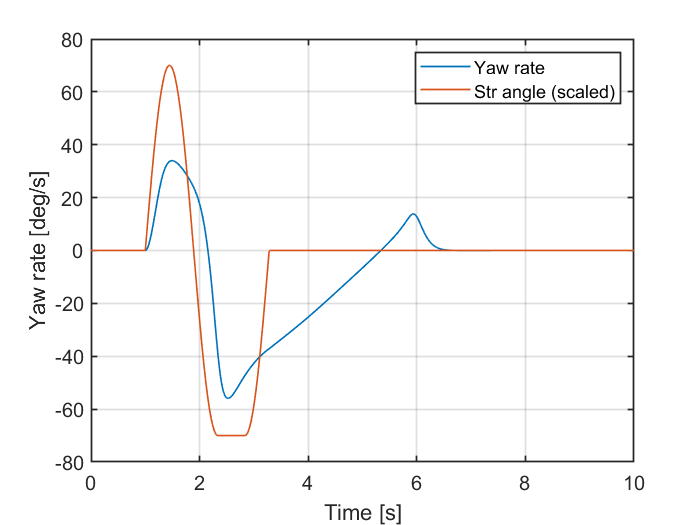
\includegraphics[width=\linewidth]{Figures/3_3_ESCoff.png}
        %  \caption*{Trajectory} 
        % \label{fig:2_4_l}
    \end{minipage} 
    \begin{minipage}[b]{0.49\linewidth}
    \centering
        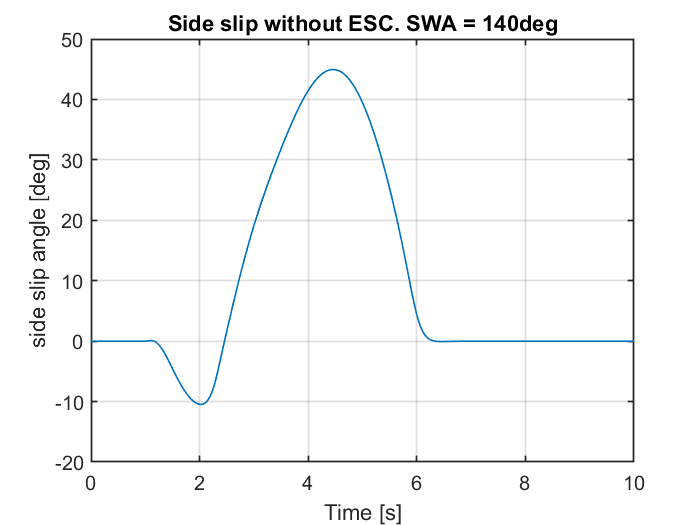
\includegraphics[width=\linewidth]{Figures/3_3_ESCoff_sideSlip.png}
        % \caption*{Yaw rate}
        % \label{fig:2_4_u}
    \end{minipage} 
    \caption{Side Slip and Yaw Rate with Load Transfer for Sine with Dwell Test}
    %  \label{fig:headbodyrelmotion}
\end{figure}

The figure above shows the simulation when the vehicle fails. The steering wheel input is $140^{\circ}$, and the vehicle fails the first and second test at the simultaneously. This means that the vehicle with load transfer is less stable than the ideal vehicle model. The reason is that upon adding load transfer, the forces on each side of the vehicle will increase or decrease respectively. This change in the $\Delta F$ will change the cornering stiffness of the vehicle and hence the handling characteristics. Generally, the cornering stiffness will increase on the outside wheels and decrease in the inside wheels due to the load transfer. However, because of the non-linearity of the tyres, the decrease is larger than the increase. Hence, the average cornering stiffness for one axle will decrease, giving the vehicle less grip. 